\section{Arquitetura}
\subsection{Arquitetura lógica}
O CliniCore é um monolito modular em Next.js (App Router) e TypeScript. Páginas, Server Actions e rotas de API pertencem à camada de interface. A camada de negócio contém a fachada, os controles, as regras, as exceções e as interfaces dos repositórios. A infraestrutura implementa essas interfaces com coleções em RAM ou SQLite por Drizzle ORM. As dependências são \textbf{ui $\rightarrow$ business $\leftarrow$ infra}; os controles não importam Drizzle nem SQLite.

\begin{figure}[H]\centering
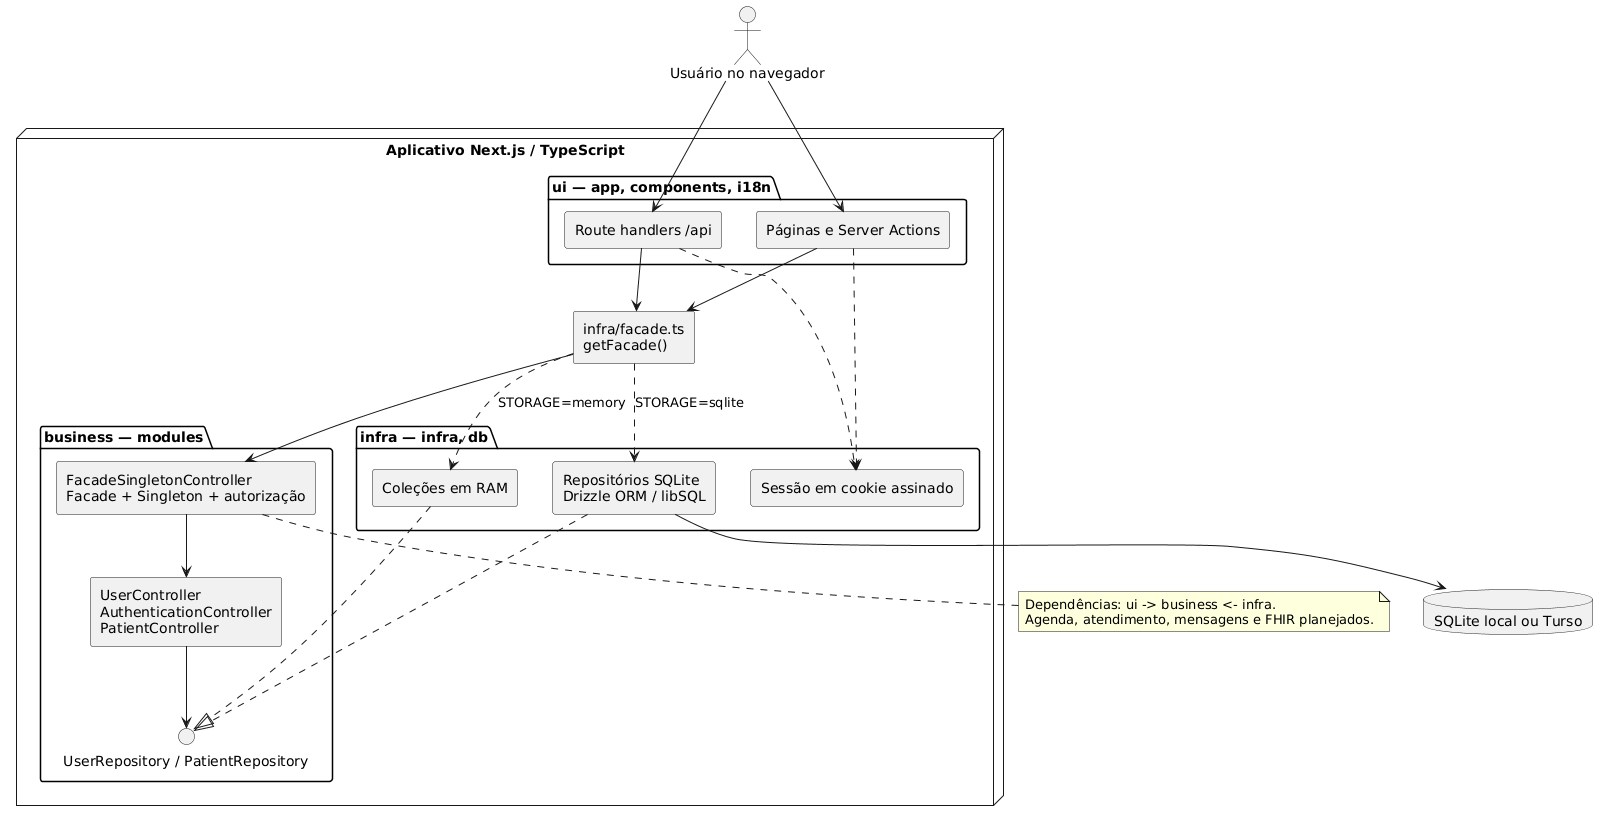
\includegraphics[width=\textwidth,height=0.75\textheight,keepaspectratio]{images/diagrama-arquitetura.png}
\caption{Arquitetura lógica implementada até a Sprint 3.}
\end{figure}

\subsection{Execução e persistência}
Na execução local, o navegador acessa o aplicativo Next.js. A variável \path|STORAGE|, lida na inicialização, seleciona \path|memory| (coleções em RAM, perdidas ao encerrar o processo) ou \path|sqlite| (banco definido por \path|DATABASE_URL|). SQLite pode usar arquivo local ou conexão libSQL com Turso. SQLite com endereço \path|:memory:| aparece nos testes de infraestrutura e não é o mecanismo RAM da aplicação.

\begin{figure}[H]\centering
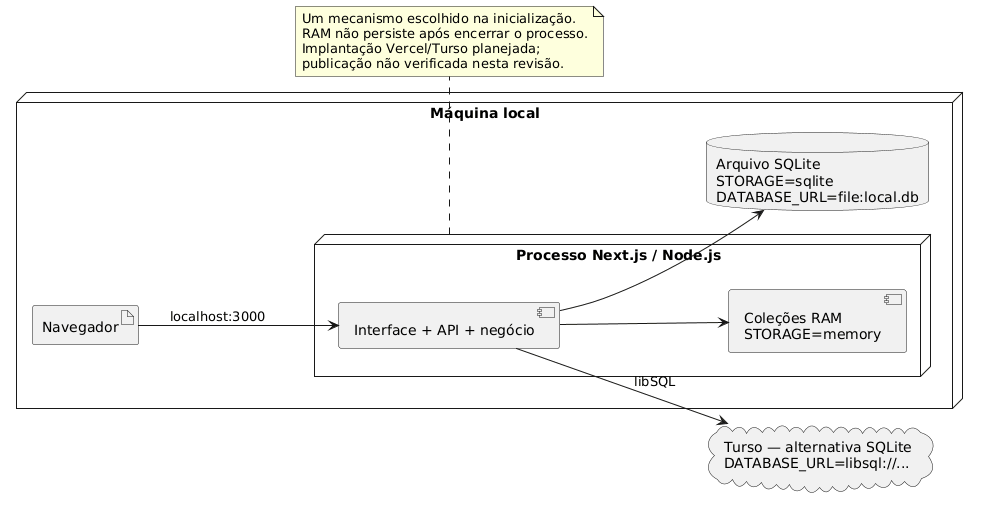
\includegraphics[width=\textwidth,height=0.65\textheight,keepaspectratio]{images/implantacao.png}
\caption{Execução local e alternativas de armazenamento.}
\end{figure}